% Options for packages loaded elsewhere
\PassOptionsToPackage{unicode}{hyperref}
\PassOptionsToPackage{hyphens}{url}
%
\documentclass[
]{article}
\usepackage{lmodern}
\usepackage{amssymb,amsmath}
\usepackage{ifxetex,ifluatex}
\ifnum 0\ifxetex 1\fi\ifluatex 1\fi=0 % if pdftex
  \usepackage[T1]{fontenc}
  \usepackage[utf8]{inputenc}
  \usepackage{textcomp} % provide euro and other symbols
\else % if luatex or xetex
  \usepackage{unicode-math}
  \defaultfontfeatures{Scale=MatchLowercase}
  \defaultfontfeatures[\rmfamily]{Ligatures=TeX,Scale=1}
\fi
% Use upquote if available, for straight quotes in verbatim environments
\IfFileExists{upquote.sty}{\usepackage{upquote}}{}
\IfFileExists{microtype.sty}{% use microtype if available
  \usepackage[]{microtype}
  \UseMicrotypeSet[protrusion]{basicmath} % disable protrusion for tt fonts
}{}
\makeatletter
\@ifundefined{KOMAClassName}{% if non-KOMA class
  \IfFileExists{parskip.sty}{%
    \usepackage{parskip}
  }{% else
    \setlength{\parindent}{0pt}
    \setlength{\parskip}{6pt plus 2pt minus 1pt}}
}{% if KOMA class
  \KOMAoptions{parskip=half}}
\makeatother
\usepackage{xcolor}
\IfFileExists{xurl.sty}{\usepackage{xurl}}{} % add URL line breaks if available
\IfFileExists{bookmark.sty}{\usepackage{bookmark}}{\usepackage{hyperref}}
\hypersetup{
  pdftitle={Simple 3-state Partitioned Survival model in R},
  pdfauthor={The DARTH workgroup},
  hidelinks,
  pdfcreator={LaTeX via pandoc}}
\urlstyle{same} % disable monospaced font for URLs
\usepackage[margin=1in]{geometry}
\usepackage{color}
\usepackage{fancyvrb}
\newcommand{\VerbBar}{|}
\newcommand{\VERB}{\Verb[commandchars=\\\{\}]}
\DefineVerbatimEnvironment{Highlighting}{Verbatim}{commandchars=\\\{\}}
% Add ',fontsize=\small' for more characters per line
\usepackage{framed}
\definecolor{shadecolor}{RGB}{248,248,248}
\newenvironment{Shaded}{\begin{snugshade}}{\end{snugshade}}
\newcommand{\AlertTok}[1]{\textcolor[rgb]{0.94,0.16,0.16}{#1}}
\newcommand{\AnnotationTok}[1]{\textcolor[rgb]{0.56,0.35,0.01}{\textbf{\textit{#1}}}}
\newcommand{\AttributeTok}[1]{\textcolor[rgb]{0.77,0.63,0.00}{#1}}
\newcommand{\BaseNTok}[1]{\textcolor[rgb]{0.00,0.00,0.81}{#1}}
\newcommand{\BuiltInTok}[1]{#1}
\newcommand{\CharTok}[1]{\textcolor[rgb]{0.31,0.60,0.02}{#1}}
\newcommand{\CommentTok}[1]{\textcolor[rgb]{0.56,0.35,0.01}{\textit{#1}}}
\newcommand{\CommentVarTok}[1]{\textcolor[rgb]{0.56,0.35,0.01}{\textbf{\textit{#1}}}}
\newcommand{\ConstantTok}[1]{\textcolor[rgb]{0.00,0.00,0.00}{#1}}
\newcommand{\ControlFlowTok}[1]{\textcolor[rgb]{0.13,0.29,0.53}{\textbf{#1}}}
\newcommand{\DataTypeTok}[1]{\textcolor[rgb]{0.13,0.29,0.53}{#1}}
\newcommand{\DecValTok}[1]{\textcolor[rgb]{0.00,0.00,0.81}{#1}}
\newcommand{\DocumentationTok}[1]{\textcolor[rgb]{0.56,0.35,0.01}{\textbf{\textit{#1}}}}
\newcommand{\ErrorTok}[1]{\textcolor[rgb]{0.64,0.00,0.00}{\textbf{#1}}}
\newcommand{\ExtensionTok}[1]{#1}
\newcommand{\FloatTok}[1]{\textcolor[rgb]{0.00,0.00,0.81}{#1}}
\newcommand{\FunctionTok}[1]{\textcolor[rgb]{0.00,0.00,0.00}{#1}}
\newcommand{\ImportTok}[1]{#1}
\newcommand{\InformationTok}[1]{\textcolor[rgb]{0.56,0.35,0.01}{\textbf{\textit{#1}}}}
\newcommand{\KeywordTok}[1]{\textcolor[rgb]{0.13,0.29,0.53}{\textbf{#1}}}
\newcommand{\NormalTok}[1]{#1}
\newcommand{\OperatorTok}[1]{\textcolor[rgb]{0.81,0.36,0.00}{\textbf{#1}}}
\newcommand{\OtherTok}[1]{\textcolor[rgb]{0.56,0.35,0.01}{#1}}
\newcommand{\PreprocessorTok}[1]{\textcolor[rgb]{0.56,0.35,0.01}{\textit{#1}}}
\newcommand{\RegionMarkerTok}[1]{#1}
\newcommand{\SpecialCharTok}[1]{\textcolor[rgb]{0.00,0.00,0.00}{#1}}
\newcommand{\SpecialStringTok}[1]{\textcolor[rgb]{0.31,0.60,0.02}{#1}}
\newcommand{\StringTok}[1]{\textcolor[rgb]{0.31,0.60,0.02}{#1}}
\newcommand{\VariableTok}[1]{\textcolor[rgb]{0.00,0.00,0.00}{#1}}
\newcommand{\VerbatimStringTok}[1]{\textcolor[rgb]{0.31,0.60,0.02}{#1}}
\newcommand{\WarningTok}[1]{\textcolor[rgb]{0.56,0.35,0.01}{\textbf{\textit{#1}}}}
\usepackage{graphicx,grffile}
\makeatletter
\def\maxwidth{\ifdim\Gin@nat@width>\linewidth\linewidth\else\Gin@nat@width\fi}
\def\maxheight{\ifdim\Gin@nat@height>\textheight\textheight\else\Gin@nat@height\fi}
\makeatother
% Scale images if necessary, so that they will not overflow the page
% margins by default, and it is still possible to overwrite the defaults
% using explicit options in \includegraphics[width, height, ...]{}
\setkeys{Gin}{width=\maxwidth,height=\maxheight,keepaspectratio}
% Set default figure placement to htbp
\makeatletter
\def\fps@figure{htbp}
\makeatother
\setlength{\emergencystretch}{3em} % prevent overfull lines
\providecommand{\tightlist}{%
  \setlength{\itemsep}{0pt}\setlength{\parskip}{0pt}}
\setcounter{secnumdepth}{-\maxdimen} % remove section numbering

\title{Simple 3-state Partitioned Survival model in R}
\author{The DARTH workgroup}
\date{}

\begin{document}
\maketitle

Developed by the Decision Analysis in R for Technologies in Health
(DARTH) workgroup:

Fernando Alarid-Escudero, PhD (1)

Eva A. Enns, MS, PhD (2)

M.G. Myriam Hunink, MD, PhD (3,4)

Hawre J. Jalal, MD, PhD (5)

Eline M. Krijkamp, MSc (3)

Petros Pechlivanoglou, PhD (6)

Alan Yang, MSc (7)

In collaboration of:

\begin{enumerate}
\def\labelenumi{\arabic{enumi}.}
\tightlist
\item
  Drug Policy Program, Center for Research and Teaching in Economics
  (CIDE) - CONACyT, Aguascalientes, Mexico
\item
  University of Minnesota School of Public Health, Minneapolis, MN, USA
\item
  Erasmus MC, Rotterdam, The Netherlands
\item
  Harvard T.H. Chan School of Public Health, Boston, USA
\item
  University of Pittsburgh Graduate School of Public Health, Pittsburgh,
  PA, USA
\item
  The Hospital for Sick Children, Toronto and University of Toronto,
  Toronto ON, Canada
\item
  The Hospital for Sick Children, Toronto ON, Canada
\end{enumerate}

Please cite our publications when using this code:

\begin{itemize}
\item
  Jalal H, Pechlivanoglou P, Krijkamp E, Alarid-Escudero F, Enns E,
  Hunink MG. An Overview of R in Health Decision Sciences. Med Decis
  Making. 2017; 37(3): 735-746.
  \url{https://journals.sagepub.com/doi/abs/10.1177/0272989X16686559}
\item
  Krijkamp EM, Alarid-Escudero F, Enns EA, Jalal HJ, Hunink MGM,
  Pechlivanoglou P. Microsimulation modeling for health decision
  sciences using R: A tutorial. Med Decis Making. 2018;38(3):400--22.
  \url{https://journals.sagepub.com/doi/abs/10.1177/0272989X18754513}
\item
  Krijkamp EM, Alarid-Escudero F, Enns E, Pechlivanoglou P, Hunink MM,
  Jalal H. A Multidimensional Array Representation of State-Transition
  Model Dynamics. BioRxiv 670612
  2019.https://www.biorxiv.org/content/10.1101/670612v1
\end{itemize}

Copyright 2017, THE HOSPITAL FOR SICK CHILDREN AND THE COLLABORATING
INSTITUTIONS. All rights reserved in Canada, the United States and
worldwide. Copyright, trademarks, trade names and any and all associated
intellectual property are exclusively owned by THE HOSPITAL FOR Sick
CHILDREN and the collaborating institutions. These materials may be
used, reproduced, modified, distributed and adapted with proper
attribution.

\newpage

\begin{Shaded}
\begin{Highlighting}[]
\KeywordTok{rm}\NormalTok{(}\DataTypeTok{list =} \KeywordTok{ls}\NormalTok{())      }\CommentTok{# clear memory (removes all the variables from the workspace)}
\end{Highlighting}
\end{Shaded}

\hypertarget{load-packages}{%
\section{01 Load packages}\label{load-packages}}

\begin{Shaded}
\begin{Highlighting}[]
\ControlFlowTok{if}\NormalTok{ (}\OperatorTok{!}\KeywordTok{require}\NormalTok{(}\StringTok{'pacman'}\NormalTok{)) }\KeywordTok{install.packages}\NormalTok{(}\StringTok{'pacman'}\NormalTok{); }\KeywordTok{library}\NormalTok{(pacman) }\CommentTok{# use this package to conveniently install other packages}
\CommentTok{# load (install if required) packages from CRAN}
\KeywordTok{p_load}\NormalTok{(}\StringTok{"here"}\NormalTok{, }\StringTok{"dplyr"}\NormalTok{, }\StringTok{"devtools"}\NormalTok{, }\StringTok{"gems"}\NormalTok{, }\StringTok{"flexsurv"}\NormalTok{, }\StringTok{"survminer"}\NormalTok{, }\StringTok{"survHE"}\NormalTok{, }\StringTok{"ggplot2"}\NormalTok{, }\StringTok{"msm"}\NormalTok{, }\StringTok{"igraph"}\NormalTok{, }\StringTok{"mstate"}\NormalTok{,   }\StringTok{"reshape2"}\NormalTok{, }\StringTok{"knitr"}\NormalTok{, }\StringTok{"diagram"}\NormalTok{)                                                  }
\end{Highlighting}
\end{Shaded}

\hypertarget{load-functions}{%
\section{02 Load functions}\label{load-functions}}

\begin{Shaded}
\begin{Highlighting}[]
\KeywordTok{source}\NormalTok{(}\StringTok{"survival_functions.R"}\NormalTok{)}
\end{Highlighting}
\end{Shaded}

\hypertarget{input-model-parameters}{%
\section{03 Input model parameters}\label{input-model-parameters}}

\begin{Shaded}
\begin{Highlighting}[]
\NormalTok{v_n       <-}\StringTok{ }\KeywordTok{c}\NormalTok{(}\StringTok{"healthy"}\NormalTok{, }\StringTok{"sick"}\NormalTok{, }\StringTok{"dead"}\NormalTok{)  }\CommentTok{# state names}
\NormalTok{n_s       <-}\StringTok{ }\KeywordTok{length}\NormalTok{(v_n)                   }\CommentTok{# No of states }
\NormalTok{n_i       <-}\StringTok{ }\DecValTok{5000}                          \CommentTok{# number of simulations }
\NormalTok{c_l       <-}\StringTok{ }\DecValTok{1} \OperatorTok{/}\StringTok{ }\DecValTok{12}                        \CommentTok{# cycle length (a month)}
\NormalTok{n_t       <-}\StringTok{ }\DecValTok{30}                            \CommentTok{# number of years (20 years)}
\NormalTok{times     <-}\StringTok{ }\KeywordTok{seq}\NormalTok{(}\DecValTok{0}\NormalTok{, n_t, c_l)              }\CommentTok{# the cycles in years}
\KeywordTok{set.seed}\NormalTok{(}\DecValTok{2020}\NormalTok{)                             }\CommentTok{# set the seed}
\end{Highlighting}
\end{Shaded}

Create a transition probability matrix with all transitions indicated
and numbered.

\begin{Shaded}
\begin{Highlighting}[]
\NormalTok{tmat <-}\StringTok{ }\KeywordTok{matrix}\NormalTok{(}\OtherTok{NA}\NormalTok{, n_s, n_s, }\DataTypeTok{dimnames =} \KeywordTok{list}\NormalTok{(v_n,v_n))}
\NormalTok{tmat[}\StringTok{"healthy"}\NormalTok{, }\StringTok{"sick"}\NormalTok{]  <-}\StringTok{ }\DecValTok{1}
\NormalTok{tmat[}\StringTok{"healthy"}\NormalTok{, }\StringTok{"dead"}\NormalTok{]  <-}\StringTok{ }\DecValTok{2}
\NormalTok{tmat[}\StringTok{"sick"}\NormalTok{   , }\StringTok{"dead"}\NormalTok{]  <-}\StringTok{ }\DecValTok{3}

\NormalTok{layout.fig <-}\StringTok{ }\KeywordTok{c}\NormalTok{(}\DecValTok{2}\NormalTok{,}\DecValTok{1}\NormalTok{)}
\KeywordTok{plotmat}\NormalTok{(}\KeywordTok{t}\NormalTok{(tmat), }\KeywordTok{t}\NormalTok{(layout.fig), }\DataTypeTok{self.cex =} \FloatTok{0.5}\NormalTok{, }\DataTypeTok{curve =} \DecValTok{0}\NormalTok{, }\DataTypeTok{arr.pos =} \FloatTok{0.76}\NormalTok{,  }
        \DataTypeTok{latex =}\NormalTok{ T, }\DataTypeTok{arr.type =} \StringTok{"curved"}\NormalTok{, }\DataTypeTok{relsize =} \FloatTok{0.85}\NormalTok{, }\DataTypeTok{box.prop=}\FloatTok{0.8}\NormalTok{, }
        \DataTypeTok{cex =} \FloatTok{0.1}\NormalTok{, }\DataTypeTok{box.cex =} \FloatTok{0.7}\NormalTok{, }\DataTypeTok{lwd =} \DecValTok{1}\NormalTok{)}
\end{Highlighting}
\end{Shaded}

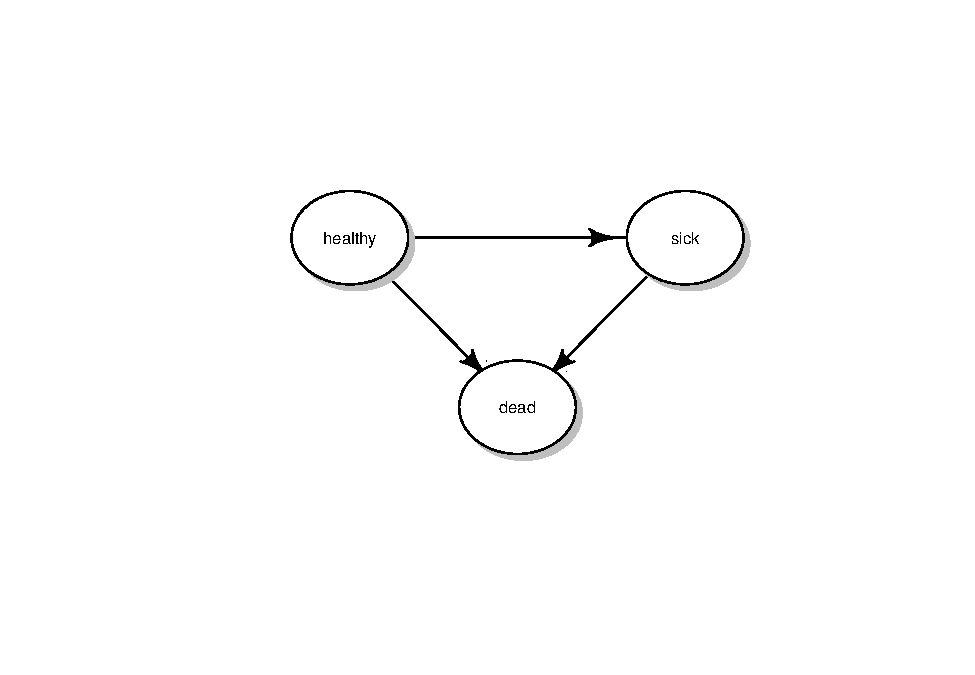
\includegraphics{survival_3-state_solutions_files/figure-latex/unnamed-chunk-5-1.pdf}

Generate data.

\begin{Shaded}
\begin{Highlighting}[]
\KeywordTok{source}\NormalTok{(}\StringTok{"data.R"}\NormalTok{)}
\end{Highlighting}
\end{Shaded}

\begin{verbatim}
## Simulating patient:1
\end{verbatim}

\begin{verbatim}
## Simulating patient:100
\end{verbatim}

\begin{verbatim}
## Simulating patient:200
\end{verbatim}

\begin{verbatim}
## Simulating patient:300
\end{verbatim}

\begin{verbatim}
## Simulating patient:400
\end{verbatim}

\begin{verbatim}
## Simulating patient:500
\end{verbatim}

\begin{Shaded}
\begin{Highlighting}[]
\KeywordTok{head}\NormalTok{(true_data)}
\end{Highlighting}
\end{Shaded}

\begin{verbatim}
##           healthy     sick      dead
## Patient 1       0 1.448160 10.650946
## Patient 2       0 2.082438  2.539559
## Patient 3       0 2.332880  3.304383
## Patient 4       0 7.613460  7.856301
## Patient 5       0 5.521759 60.000000
## Patient 6       0 4.836634 34.077378
\end{verbatim}

\begin{Shaded}
\begin{Highlighting}[]
\KeywordTok{head}\NormalTok{(sim_data)}
\end{Highlighting}
\end{Shaded}

\begin{verbatim}
##           healthy      sick      dead
## Patient 1       0 1.4481602 4.6703210
## Patient 2       0 0.2330877 0.2330877
## Patient 3       0 2.3328803 3.3043830
## Patient 4       0 5.0000000 5.0000000
## Patient 5       0 1.1391762 1.1391762
## Patient 6       0 4.8366340 5.0000000
\end{verbatim}

\begin{Shaded}
\begin{Highlighting}[]
\KeywordTok{head}\NormalTok{(status)}
\end{Highlighting}
\end{Shaded}

\begin{verbatim}
##   healthy sick dead
## 1       1    1    0
## 2       1    0    0
## 3       1    1    1
## 4       1    0    0
## 5       1    0    0
## 6       1    1    0
\end{verbatim}

\begin{Shaded}
\begin{Highlighting}[]
\KeywordTok{head}\NormalTok{(OS_PFS_data)}
\end{Highlighting}
\end{Shaded}

\begin{verbatim}
##    PFS_time PFS_status   OS_time OS_status
## 1 1.4481602          1 4.6703210         0
## 2 0.2330877          0 0.2330877         0
## 3 2.3328803          1 3.3043830         1
## 4 5.0000000          0 5.0000000         0
## 5 1.1391762          0 1.1391762         0
## 6 4.8366340          1 5.0000000         0
\end{verbatim}

\hypertarget{analysis}{%
\section{04 Analysis}\label{analysis}}

Showcasing the use of packages \texttt{survival}, \texttt{flexsurv}.

\begin{Shaded}
\begin{Highlighting}[]
\NormalTok{fit_KM   <-}\StringTok{ }\KeywordTok{survfit}\NormalTok{(}\KeywordTok{Surv}\NormalTok{(}\DataTypeTok{time =}\NormalTok{ OS_time, }\DataTypeTok{event =}\NormalTok{ OS_status) }\OperatorTok{~}\StringTok{ }\DecValTok{1}\NormalTok{, }\DataTypeTok{data =}\NormalTok{ OS_PFS_data, }
                         \DataTypeTok{type =}\StringTok{"fleming-harrington"}\NormalTok{)}
\KeywordTok{plot}\NormalTok{(fit_KM, }\DataTypeTok{mark.time =}\NormalTok{ T)}


\CommentTok{# a prettier way of plotting!!}

\KeywordTok{ggsurvplot}\NormalTok{(}
\NormalTok{  fit_KM, }
  \DataTypeTok{data =}\NormalTok{ OS_PFS_data, }
  \DataTypeTok{size =} \DecValTok{1}\NormalTok{,                  }\CommentTok{# change line size}
  \DataTypeTok{palette =} \KeywordTok{c}\NormalTok{(}\StringTok{"orange2"}\NormalTok{),    }\CommentTok{# custom color palettes}
  \DataTypeTok{conf.int =} \OtherTok{TRUE}\NormalTok{,           }\CommentTok{# Add confidence interval}
  \DataTypeTok{pval =} \OtherTok{TRUE}\NormalTok{,               }\CommentTok{# Add p-value}
  \DataTypeTok{risk.table =} \OtherTok{TRUE}\NormalTok{,         }\CommentTok{# Add risk table}
  \DataTypeTok{risk.table.height =} \FloatTok{0.25}\NormalTok{,  }\CommentTok{# Useful to change when you have multiple groups}
  \DataTypeTok{ggtheme =} \KeywordTok{theme_bw}\NormalTok{(),      }\CommentTok{# Change ggplot2 theme}
  \DataTypeTok{xlab =} \StringTok{'Time in days'}\NormalTok{,     }\CommentTok{# Change X-axis label}
  \DataTypeTok{title    =} \StringTok{"Survival curve for Progression-Free Survival (PFS)"}\NormalTok{, }
  \DataTypeTok{subtitle =} \StringTok{"Based on Kaplan-Meier estimates"}
\NormalTok{) }
\end{Highlighting}
\end{Shaded}

\begin{verbatim}
## Warning in .pvalue(fit, data = data, method = method, pval = pval, pval.coord = pval.coord, : There are no survival curves to be compared. 
##  This is a null model.
\end{verbatim}

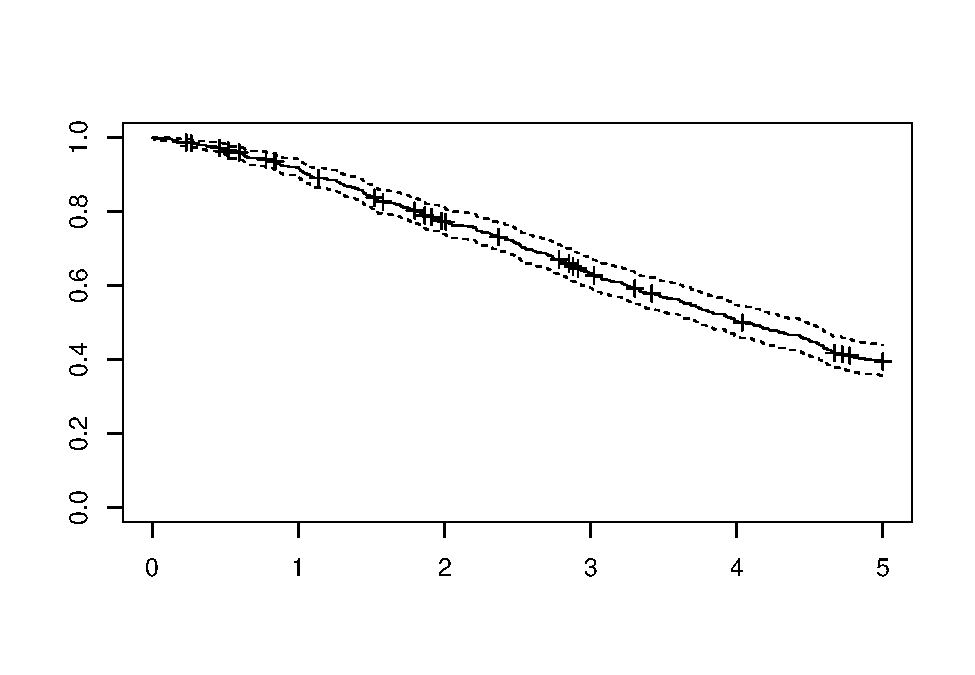
\includegraphics{survival_3-state_solutions_files/figure-latex/unnamed-chunk-7-1.pdf}
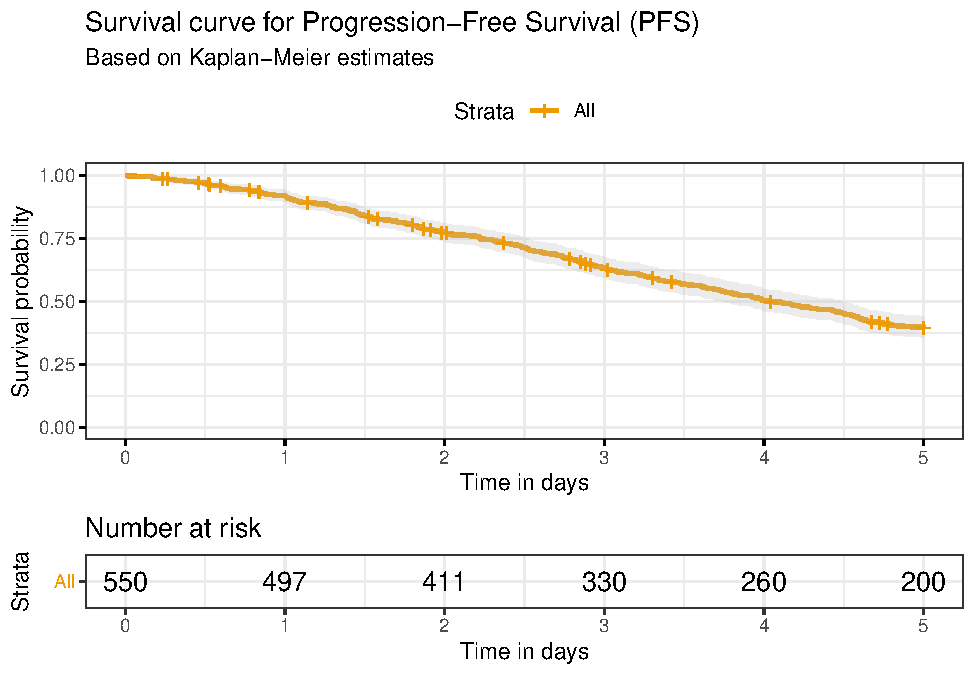
\includegraphics{survival_3-state_solutions_files/figure-latex/unnamed-chunk-7-2.pdf}

\hypertarget{partitioned-survival-model}{%
\subsection{04.1 Partitioned Survival
model}\label{partitioned-survival-model}}

\begin{Shaded}
\begin{Highlighting}[]
\CommentTok{# Flexsurv allows parametric fitting of curves}
\NormalTok{fit_weib <-}\StringTok{ }\KeywordTok{flexsurvreg}\NormalTok{(}\KeywordTok{Surv}\NormalTok{(}\DataTypeTok{time =}\NormalTok{ OS_time, }\DataTypeTok{event =}\NormalTok{ OS_status) }\OperatorTok{~}\StringTok{ }\DecValTok{1}\NormalTok{, }\DataTypeTok{data =}\NormalTok{ OS_PFS_data,  }\DataTypeTok{dist =} \StringTok{"weibull"}\NormalTok{)}
\KeywordTok{plot}\NormalTok{(fit_weib)}
\end{Highlighting}
\end{Shaded}

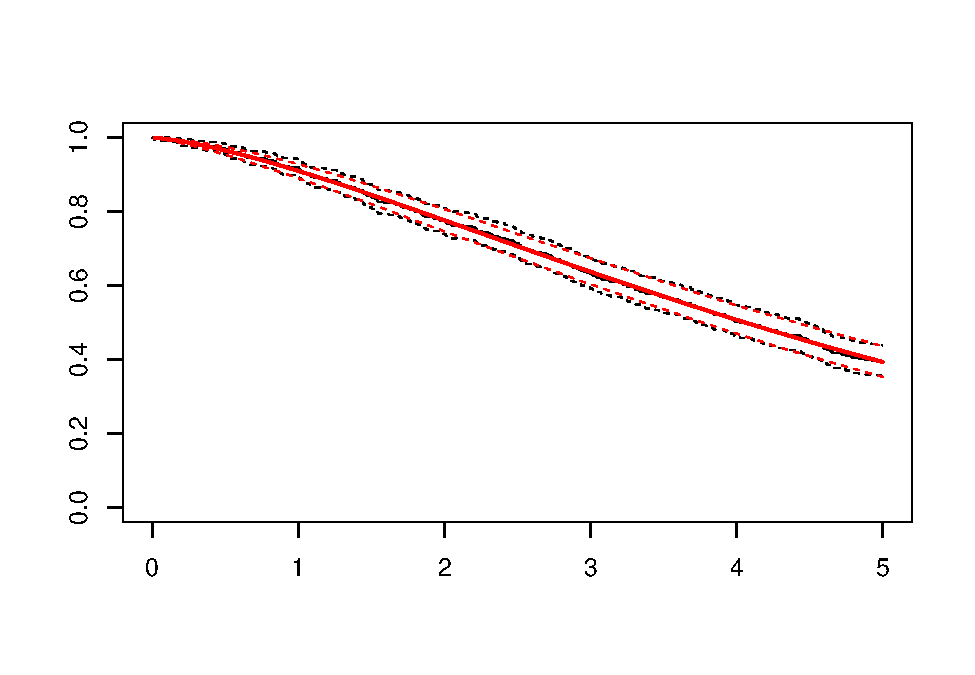
\includegraphics{survival_3-state_solutions_files/figure-latex/unnamed-chunk-8-1.pdf}

\begin{Shaded}
\begin{Highlighting}[]
\CommentTok{# fit all parametric models to the data and extract the AIC/BIC. }
\CommentTok{# Select the one with the most appropriate fit}
\CommentTok{# Repeat for PFS and OS}




\NormalTok{fit_PFS  <-}\StringTok{ }\KeywordTok{fit.fun}\NormalTok{(}\DataTypeTok{time  =} \StringTok{"PFS_time"}\NormalTok{, }\DataTypeTok{status =} \StringTok{"PFS_status"}\NormalTok{, }\DataTypeTok{data =}\NormalTok{ OS_PFS_data, }
                    \DataTypeTok{times =}\NormalTok{ times, }\DataTypeTok{extrapolate =}\NormalTok{ T) }
\end{Highlighting}
\end{Shaded}

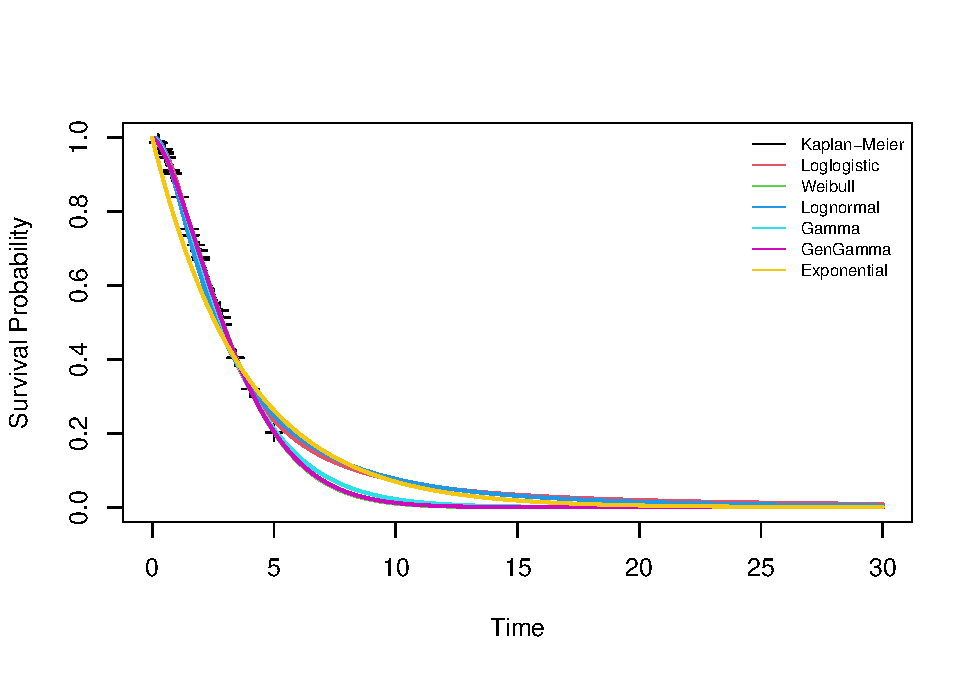
\includegraphics{survival_3-state_solutions_files/figure-latex/unnamed-chunk-8-2.pdf}

\begin{Shaded}
\begin{Highlighting}[]
\NormalTok{fit_OS   <-}\StringTok{ }\KeywordTok{fit.fun}\NormalTok{(}\DataTypeTok{time  =} \StringTok{"OS_time"}\NormalTok{, }\DataTypeTok{status  =} \StringTok{"OS_status"}\NormalTok{ , }\DataTypeTok{data =}\NormalTok{ OS_PFS_data, }
                    \DataTypeTok{times =}\NormalTok{ times, }\DataTypeTok{extrapolate =}\NormalTok{ T) }
\end{Highlighting}
\end{Shaded}

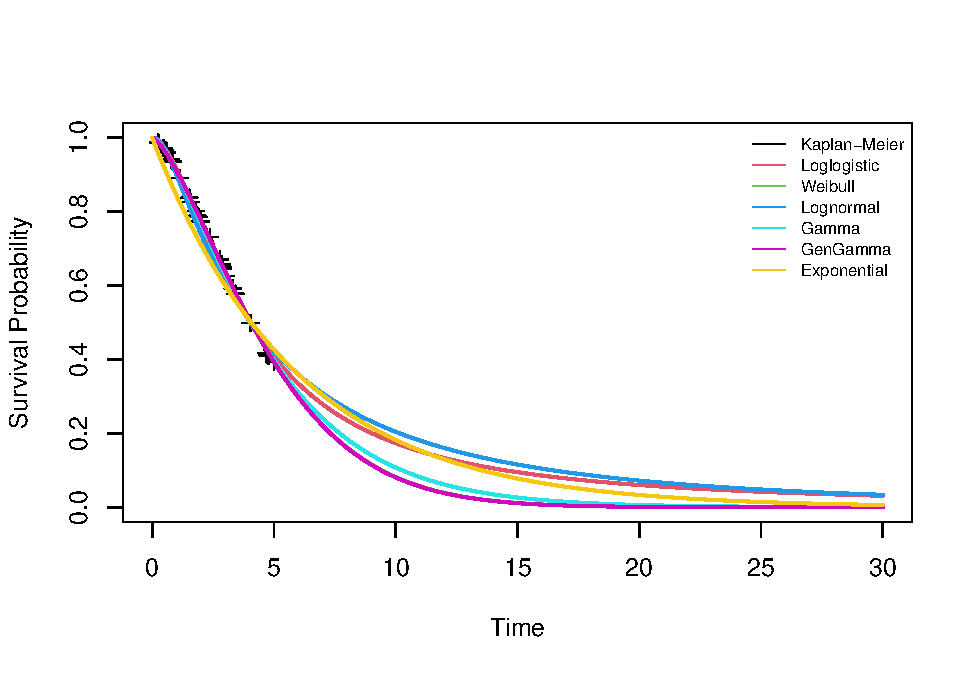
\includegraphics{survival_3-state_solutions_files/figure-latex/unnamed-chunk-8-3.pdf}

\begin{Shaded}
\begin{Highlighting}[]
\NormalTok{best_PFS <-}\StringTok{ }\NormalTok{fit_PFS[[}\StringTok{"Weibull"}\NormalTok{]]  }
\NormalTok{best_OS  <-}\StringTok{ }\NormalTok{fit_OS [[}\StringTok{"Weibull"}\NormalTok{]]}

\CommentTok{# construct a partitioned survival model out of the fitted models}
\NormalTok{m_M_PSM <-}\StringTok{ }\KeywordTok{partsurv}\NormalTok{(best_PFS, best_OS, }\DataTypeTok{time =}\NormalTok{ times)}\OperatorTok{$}\NormalTok{trace}
\end{Highlighting}
\end{Shaded}

\hypertarget{multistate-modeling-method-1}{%
\subsection{04.2 MultiState modeling method
1}\label{multistate-modeling-method-1}}

\begin{itemize}
\tightlist
\item
  Fit all parametric multistate models simultaneously.
\end{itemize}

\begin{Shaded}
\begin{Highlighting}[]
\CommentTok{# The existing functions in R require the data in a long rather than a wide format}
\CommentTok{# convert the data in a way that flexsurv understands using the mstate package}
\NormalTok{data_long       <-}\StringTok{ }\KeywordTok{msprep}\NormalTok{(}\DataTypeTok{time =}\NormalTok{ sim_data, }\DataTypeTok{status =}\NormalTok{ status, }\DataTypeTok{trans =}\NormalTok{ tmat )}
\NormalTok{data_long}\OperatorTok{$}\NormalTok{trans <-}\StringTok{ }\KeywordTok{as.factor}\NormalTok{(data_long}\OperatorTok{$}\NormalTok{trans) }\CommentTok{# convert trans to a factor}

\NormalTok{data_long}\OperatorTok{$}\NormalTok{from  <-}\StringTok{ }\KeywordTok{case_when}\NormalTok{(data_long}\OperatorTok{$}\NormalTok{from }\OperatorTok{==}\StringTok{ }\DecValTok{1} \OperatorTok{~}\StringTok{ "healthy"}\NormalTok{,}
\NormalTok{                             data_long}\OperatorTok{$}\NormalTok{from }\OperatorTok{==}\StringTok{ }\DecValTok{2} \OperatorTok{~}\StringTok{ "sick"}\NormalTok{,}
\NormalTok{                             data_long}\OperatorTok{$}\NormalTok{from }\OperatorTok{==}\StringTok{ }\DecValTok{3} \OperatorTok{~}\StringTok{ "dead"}\NormalTok{)}

\NormalTok{data_long}\OperatorTok{$}\NormalTok{to    <-}\StringTok{ }\KeywordTok{case_when}\NormalTok{(data_long}\OperatorTok{$}\NormalTok{to }\OperatorTok{==}\StringTok{ }\DecValTok{1} \OperatorTok{~}\StringTok{ "healthy"}\NormalTok{, }
\NormalTok{                             data_long}\OperatorTok{$}\NormalTok{to }\OperatorTok{==}\StringTok{ }\DecValTok{2} \OperatorTok{~}\StringTok{ "sick"}\NormalTok{,}
\NormalTok{                             data_long}\OperatorTok{$}\NormalTok{to }\OperatorTok{==}\StringTok{ }\DecValTok{3} \OperatorTok{~}\StringTok{ "dead"}\NormalTok{)}

\CommentTok{# fit all parametric multistate models simultaneously to the data and extract the AIC/BIC }
\CommentTok{# Select the one with the lowest AIC}
\NormalTok{fits <-}\StringTok{ }\KeywordTok{fit.mstate}\NormalTok{(}\DataTypeTok{time =}\StringTok{"time"}\NormalTok{, }\DataTypeTok{status =} \StringTok{"status"}\NormalTok{, trans, }\DataTypeTok{data =}\NormalTok{ data_long, }
                   \DataTypeTok{times =}\NormalTok{ times, }\DataTypeTok{extrapolate =}\NormalTok{ T )}
\end{Highlighting}
\end{Shaded}

\begin{verbatim}
## Warning in (function (q, shape, rate = 1, scale = 1/rate, lower.tail = TRUE, :
## NaNs produced
\end{verbatim}

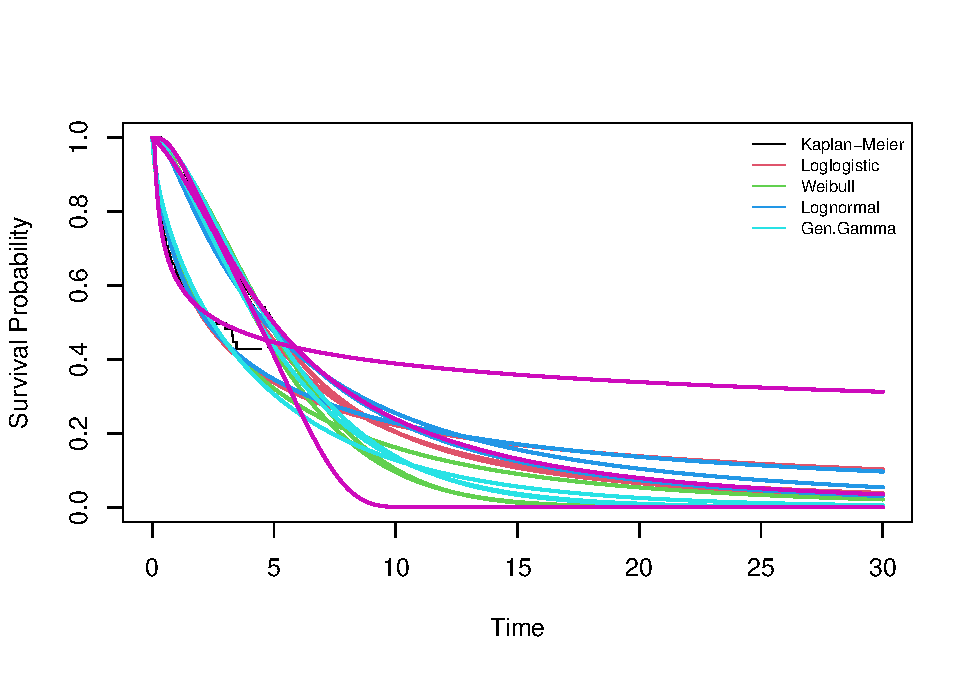
\includegraphics{survival_3-state_solutions_files/figure-latex/unnamed-chunk-9-1.pdf}

\begin{Shaded}
\begin{Highlighting}[]
\NormalTok{best.fit <-}\StringTok{ }\NormalTok{fits[[}\StringTok{"Loglogistic"}\NormalTok{]]}
\end{Highlighting}
\end{Shaded}

\begin{itemize}
\tightlist
\item
  Construct a DES model out of the simultaneously fitted multistate
  model.
\end{itemize}

\begin{Shaded}
\begin{Highlighting}[]
\CommentTok{# Construct a DES model out of the simultaneously fitted multistate model}
\NormalTok{DES_data <-}\StringTok{ }\KeywordTok{sim.fmsm}\NormalTok{(best.fit, }\DataTypeTok{start =} \DecValTok{1}\NormalTok{, }\DataTypeTok{t =}\NormalTok{ n_years, }\DataTypeTok{trans =}\NormalTok{ tmat, }\DataTypeTok{M =}\NormalTok{ n_i)}
\NormalTok{m_M_DES  <-}\StringTok{ }\KeywordTok{trace.DES}\NormalTok{(DES_data, }\DataTypeTok{n_i  =}\NormalTok{ n_i , }\DataTypeTok{times =}\NormalTok{ times, }\DataTypeTok{tmat =}\NormalTok{ tmat)}
\end{Highlighting}
\end{Shaded}

\hypertarget{multistate-modeling-method-2}{%
\subsection{04.3 MultiState modeling method
2}\label{multistate-modeling-method-2}}

\begin{itemize}
\tightlist
\item
  Multistate models can be fitted independently for each transition.
\end{itemize}

\begin{Shaded}
\begin{Highlighting}[]
\CommentTok{# Multistate models can be fitted independently for each transition.This is more flexible!}
\CommentTok{# Create subsets for each transition}
\NormalTok{data_HS <-}\StringTok{ }\KeywordTok{subset}\NormalTok{(data_long, trans }\OperatorTok{==}\StringTok{ }\DecValTok{1}\NormalTok{)}
\NormalTok{data_HD <-}\StringTok{ }\KeywordTok{subset}\NormalTok{(data_long, trans }\OperatorTok{==}\StringTok{ }\DecValTok{2}\NormalTok{)}
\NormalTok{data_SD <-}\StringTok{ }\KeywordTok{subset}\NormalTok{(data_long, trans }\OperatorTok{==}\StringTok{ }\DecValTok{3}\NormalTok{)}


\CommentTok{# fit independent models for each transition and pick the one with the lowest AIC}
\NormalTok{fit_HS <-}\StringTok{ }\KeywordTok{fit.fun}\NormalTok{(}\DataTypeTok{time =} \StringTok{"time"}\NormalTok{, }\DataTypeTok{status =} \StringTok{"status"}\NormalTok{, }\DataTypeTok{data =}\NormalTok{ data_HS, }\DataTypeTok{times =}\NormalTok{ times, }
                  \DataTypeTok{extrapolate =}\NormalTok{ T)}
\end{Highlighting}
\end{Shaded}

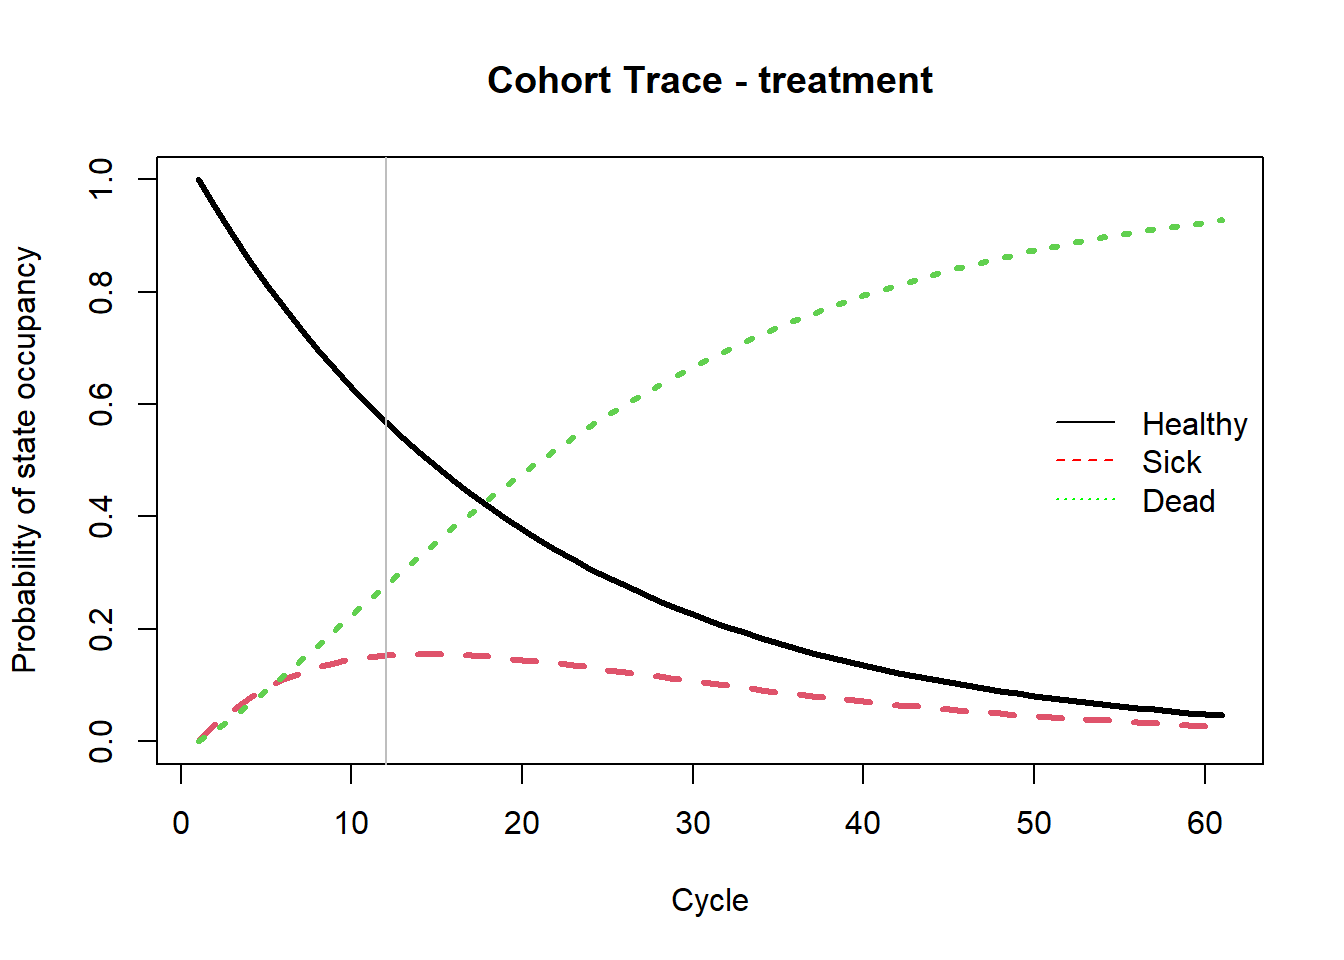
\includegraphics{survival_3-state_solutions_files/figure-latex/unnamed-chunk-11-1.pdf}

\begin{Shaded}
\begin{Highlighting}[]
\NormalTok{fit_HD <-}\StringTok{ }\KeywordTok{fit.fun}\NormalTok{(}\DataTypeTok{time =} \StringTok{"time"}\NormalTok{, }\DataTypeTok{status =} \StringTok{"status"}\NormalTok{, }\DataTypeTok{data =}\NormalTok{ data_HD, }\DataTypeTok{times =}\NormalTok{ times, }
                  \DataTypeTok{extrapolate =}\NormalTok{ T)}
\end{Highlighting}
\end{Shaded}

\includegraphics{survival_3-state_solutions_files/figure-latex/unnamed-chunk-11-2.pdf}

\begin{Shaded}
\begin{Highlighting}[]
\NormalTok{fit_SD <-}\StringTok{ }\KeywordTok{fit.fun}\NormalTok{(}\DataTypeTok{time =} \StringTok{"time"}\NormalTok{, }\DataTypeTok{status =} \StringTok{"status"}\NormalTok{, }\DataTypeTok{data =}\NormalTok{ data_SD, }\DataTypeTok{times =}\NormalTok{ times, }
                  \DataTypeTok{extrapolate =}\NormalTok{ T)}
\end{Highlighting}
\end{Shaded}

\includegraphics{survival_3-state_solutions_files/figure-latex/unnamed-chunk-11-3.pdf}

\begin{Shaded}
\begin{Highlighting}[]
\NormalTok{best.fit_HS <-}\StringTok{ }\NormalTok{fit_HS[[}\StringTok{"Gamma"}\NormalTok{]]}
\NormalTok{best.fit_HD <-}\StringTok{ }\NormalTok{fit_HD[[}\StringTok{"Weibull"}\NormalTok{]]}
\NormalTok{best.fit_SD <-}\StringTok{ }\NormalTok{fit_SD[[}\StringTok{"Lognormal"}\NormalTok{]]}
\end{Highlighting}
\end{Shaded}

\begin{itemize}
\tightlist
\item
  A microsimulation can be fitted instead of a DES.
\item
  more computationally expensive but it provides more freedom to the
  modeller.
\item
  For the Microsimulation to be run, we need transition probabilities
  per unit of time.
\end{itemize}

\begin{Shaded}
\begin{Highlighting}[]
\CommentTok{# Extract transition probabilities from the best fitting models}
\NormalTok{p_HS <-}\StringTok{ }\KeywordTok{flexsurvreg_prob}\NormalTok{(}\DataTypeTok{object =}\NormalTok{ best.fit_HS, }\DataTypeTok{times =}\NormalTok{ times)}
\NormalTok{p_HD <-}\StringTok{ }\KeywordTok{flexsurvreg_prob}\NormalTok{(}\DataTypeTok{object =}\NormalTok{ best.fit_HD, }\DataTypeTok{times =}\NormalTok{ times)}
\NormalTok{p_SD <-}\StringTok{ }\KeywordTok{flexsurvreg_prob}\NormalTok{(}\DataTypeTok{object =}\NormalTok{ best.fit_SD, }\DataTypeTok{times =}\NormalTok{ times)}

\CommentTok{# everyone starts in the "healthy" state and therefore has not spent time in "sick"}
\NormalTok{v_M_init  <-}\StringTok{ }\KeywordTok{rep}\NormalTok{(}\StringTok{"healthy"}\NormalTok{, }\DataTypeTok{times =}\NormalTok{ n_i)   }
\NormalTok{v_Ts_init <-}\StringTok{ }\KeywordTok{rep}\NormalTok{(}\DecValTok{0}\NormalTok{, n_i)  }\CommentTok{# a vector with the time of being sick at the start of the model }

\CommentTok{# function that generates the transition probabilities per cycle}
\NormalTok{Probs <-}\StringTok{ }\ControlFlowTok{function}\NormalTok{(M_t, v_Ts, t) \{ }
  \CommentTok{# Arguments:}
    \CommentTok{# M_t: health state occupied by at cycle t (character variable)}
    \CommentTok{# v_Ts: vector with the duration of being sick}
    \CommentTok{# t:     current cycle }
  \CommentTok{# Returns: }
    \CommentTok{# transition probabilities for that cycle}
  
  \CommentTok{# create matrix of state transition probabilities}
\NormalTok{  m_p_t           <-}\StringTok{ }\KeywordTok{matrix}\NormalTok{(}\DecValTok{0}\NormalTok{, }\DataTypeTok{nrow =}\NormalTok{ n_s, }\DataTypeTok{ncol =}\NormalTok{ n_i) }
  \CommentTok{# give the state names to the rows}
  \KeywordTok{rownames}\NormalTok{(m_p_t) <-}\StringTok{  }\NormalTok{v_n                              }
  
  \CommentTok{# update m_p_t with the appropriate probabilities   }
  \CommentTok{# transition probabilities when healthy }
\NormalTok{  m_p_t[, M_t }\OperatorTok{==}\StringTok{ "healthy"}\NormalTok{] <-}\StringTok{ }\KeywordTok{rbind}\NormalTok{(}\DecValTok{1} \OperatorTok{-}\StringTok{ }\NormalTok{p_HD[t] }\OperatorTok{-}\StringTok{ }\NormalTok{p_HS[t], p_HS[t], p_HD[t])    }
  \CommentTok{# transition probabilities when sick }
\NormalTok{  m_p_t[, M_t }\OperatorTok{==}\StringTok{ "sick"}\NormalTok{]    <-}\StringTok{ }\KeywordTok{rbind}\NormalTok{(}\DecValTok{0}\NormalTok{, }\DecValTok{1} \OperatorTok{-}\StringTok{ }\NormalTok{p_SD[v_Ts], p_SD[v_Ts])  }
  \CommentTok{# transition probabilities when dead     }
\NormalTok{  m_p_t[, M_t }\OperatorTok{==}\StringTok{ "dead"}\NormalTok{]    <-}\StringTok{ }\KeywordTok{rbind}\NormalTok{(}\DecValTok{0}\NormalTok{, }\DecValTok{0}\NormalTok{, }\DecValTok{1}\NormalTok{)                            }
  \KeywordTok{return}\NormalTok{(}\KeywordTok{t}\NormalTok{(m_p_t))}
\NormalTok{\}       }
\end{Highlighting}
\end{Shaded}

\hypertarget{run-microsimulation}{%
\subsection{04.3.1 Run Microsimulation}\label{run-microsimulation}}

\begin{Shaded}
\begin{Highlighting}[]
\NormalTok{MicroSim <-}\StringTok{ }\ControlFlowTok{function}\NormalTok{(n_i,  }\DataTypeTok{seed =} \DecValTok{1}\NormalTok{) \{}
  \CommentTok{# Arguments:  }
  \CommentTok{# n_i:     number of individuals}
  \CommentTok{# seed:    default is 1}
  
  \KeywordTok{set.seed}\NormalTok{(seed) }\CommentTok{# set the seed}
  
  \CommentTok{# m_M is used to store the health state information over time for every individual}
\NormalTok{  times     <-}\StringTok{ }\KeywordTok{seq}\NormalTok{(}\DecValTok{0}\NormalTok{, n_t, c_l)  }\CommentTok{# the cycles in years}
  
\NormalTok{  m_M  <-}\StringTok{  }\KeywordTok{matrix}\NormalTok{(}\DataTypeTok{nrow =}\NormalTok{ n_i, }\DataTypeTok{ncol =} \KeywordTok{length}\NormalTok{(times) , }
                  \DataTypeTok{dimnames =} \KeywordTok{list}\NormalTok{(}\KeywordTok{paste}\NormalTok{(}\StringTok{"ind"}\NormalTok{ , }\DecValTok{1}\OperatorTok{:}\NormalTok{n_i, }\DataTypeTok{sep =} \StringTok{" "}\NormalTok{), }
                                  \KeywordTok{paste}\NormalTok{(}\StringTok{"year"}\NormalTok{, times, }\DataTypeTok{sep =} \StringTok{" "}\NormalTok{)))  }

\NormalTok{  m_M[, }\DecValTok{1}\NormalTok{] <-}\StringTok{ }\NormalTok{v_M_init           }\CommentTok{# initial health state for individual i}
\NormalTok{  v_Ts     <-}\StringTok{ }\NormalTok{v_Ts_init          }\CommentTok{# initialize time since illness onset for individual i}
  
  \CommentTok{# open a loop for time running cycles 1 to n_t }
  \ControlFlowTok{for}\NormalTok{ (t }\ControlFlowTok{in} \DecValTok{1}\OperatorTok{:}\NormalTok{(}\KeywordTok{length}\NormalTok{(times)}\OperatorTok{-}\DecValTok{1}\NormalTok{)) \{}
    \CommentTok{# calculate the transition probabilities for the cycle based on health state t}
\NormalTok{    m_p <-}\StringTok{ }\KeywordTok{Probs}\NormalTok{(m_M[, t], v_Ts, t)  }
    \CommentTok{# sample the current health state and store that state in matrix m_M }
\NormalTok{    m_M[, t }\OperatorTok{+}\StringTok{ }\DecValTok{1}\NormalTok{]  <-}\StringTok{ }\KeywordTok{samplev}\NormalTok{(m_p, }\DecValTok{1}\NormalTok{) }
    
    \CommentTok{# update time since illness onset for t + 1 }
\NormalTok{    v_Ts <-}\StringTok{ }\KeywordTok{ifelse}\NormalTok{(m_M[, t }\OperatorTok{+}\StringTok{ }\DecValTok{1}\NormalTok{] }\OperatorTok{==}\StringTok{ "sick"}\NormalTok{, v_Ts }\OperatorTok{+}\StringTok{ }\DecValTok{1}\NormalTok{, }\DecValTok{0}\NormalTok{) }
    
    \CommentTok{# Display simulation progress}
    \ControlFlowTok{if}\NormalTok{(t }\OperatorTok\StringTok{ }\KeywordTok{seq}\NormalTok{(}\DecValTok{1}\NormalTok{,(}\KeywordTok{length}\NormalTok{(times)),}\DecValTok{10}\NormalTok{)) \{ }\CommentTok{# display progress every 10%}
      \KeywordTok{cat}\NormalTok{(}\StringTok{'}\CharTok{\textbackslash{}r}\StringTok{'}\NormalTok{, }\KeywordTok{paste}\NormalTok{(}\KeywordTok{round}\NormalTok{(t}\OperatorTok{/}\KeywordTok{length}\NormalTok{(times)}\OperatorTok{*}\DecValTok{100}\NormalTok{,}\DecValTok{0}\NormalTok{), }\StringTok{"% done"}\NormalTok{, }\DataTypeTok{sep =} \StringTok{" "}\NormalTok{))}
\NormalTok{    \} }\ControlFlowTok{else} \ControlFlowTok{if}\NormalTok{ (t }\OperatorTok{==}\StringTok{ }\NormalTok{(}\KeywordTok{length}\NormalTok{(times)}\OperatorTok{-}\DecValTok{1}\NormalTok{)) \{}\KeywordTok{cat}\NormalTok{(}\StringTok{'}\CharTok{\textbackslash{}r}\StringTok{'}\NormalTok{, }\KeywordTok{paste}\NormalTok{(}\StringTok{"100% done"}\NormalTok{))\}}
      
\NormalTok{  \} }\CommentTok{# close the loop for the time points }
  
  \CommentTok{# store the results from the simulation in a list}
\NormalTok{  results <-}\StringTok{ }\KeywordTok{list}\NormalTok{(}\DataTypeTok{m_M =}\NormalTok{ m_M)   }
  
  \KeywordTok{return}\NormalTok{(results)  }\CommentTok{# return the results}

\NormalTok{\} }\CommentTok{# end of the MicroSim function  }

\CommentTok{# Run the simulation model}
\NormalTok{Micro_data <-}\StringTok{ }\KeywordTok{MicroSim}\NormalTok{(n_i, }\DataTypeTok{seed =} \DecValTok{1}\NormalTok{)}

\CommentTok{# create the microsimulation trace}
\NormalTok{m_M_Micro <-}\StringTok{ }\KeywordTok{t}\NormalTok{(}\KeywordTok{apply}\NormalTok{(Micro_data}\OperatorTok{$}\NormalTok{m_M, }\DecValTok{2}\NormalTok{, }\ControlFlowTok{function}\NormalTok{(x) }\KeywordTok{table}\NormalTok{(}\KeywordTok{factor}\NormalTok{(x, }\DataTypeTok{levels =}\NormalTok{ v_n, }
                                                                 \DataTypeTok{ordered =} \OtherTok{TRUE}\NormalTok{)))) }
\NormalTok{m_M_Micro <-}\StringTok{ }\NormalTok{m_M_Micro }\OperatorTok{/}\StringTok{ }\NormalTok{n_i    }\CommentTok{# calculate the proportion of individuals }
\KeywordTok{colnames}\NormalTok{(m_M_Micro) <-}\StringTok{ }\NormalTok{v_n      }
\KeywordTok{rownames}\NormalTok{(m_M_Micro) <-}\StringTok{ }\KeywordTok{paste}\NormalTok{(}\StringTok{"Cycle"}\NormalTok{, times, }\DataTypeTok{sep =} \StringTok{" "}\NormalTok{)  }
\end{Highlighting}
\end{Shaded}

\hypertarget{compare-all-methods}{%
\section{05 Compare all methods}\label{compare-all-methods}}

\begin{Shaded}
\begin{Highlighting}[]
\CommentTok{# Calculate trace for the real data}
\NormalTok{m_M_data <-}\StringTok{ }\KeywordTok{transitionProbabilities}\NormalTok{(generate}\OperatorTok{$}\NormalTok{cohort, }\DataTypeTok{times =}\NormalTok{ times)}\OperatorTok{@}\NormalTok{probabilities}

\CommentTok{# visually compare all methods}
\KeywordTok{matplot}\NormalTok{(times,m_M_data, }\DataTypeTok{type=}\StringTok{'l'}\NormalTok{, }\DataTypeTok{lty =} \DecValTok{1}\NormalTok{, }\DataTypeTok{col =} \DecValTok{1}\NormalTok{, }\DataTypeTok{ylab=} \StringTok{"proportion of cohort"}\NormalTok{, }\DataTypeTok{xlab =} \StringTok{"Time"}\NormalTok{,}
        \DataTypeTok{main =} \StringTok{"Trace comparisons"}\NormalTok{,}\DataTypeTok{xlim=}\KeywordTok{c}\NormalTok{(}\DecValTok{0}\NormalTok{,}\DecValTok{25}\NormalTok{))}
\KeywordTok{matlines}\NormalTok{(times, m_M_DES,   }\DataTypeTok{col =} \DecValTok{2}\NormalTok{, }\DataTypeTok{lty =} \DecValTok{1}\NormalTok{)}
\KeywordTok{matlines}\NormalTok{(times, m_M_Micro, }\DataTypeTok{col =} \DecValTok{3}\NormalTok{, }\DataTypeTok{lty =} \DecValTok{1}\NormalTok{)}
\KeywordTok{matlines}\NormalTok{(times, m_M_PSM,   }\DataTypeTok{col =} \DecValTok{4}\NormalTok{, }\DataTypeTok{lty =} \DecValTok{1}\NormalTok{)}
\KeywordTok{legend}\NormalTok{(}\StringTok{"right"}\NormalTok{, }\KeywordTok{c}\NormalTok{(}\StringTok{"True Data"}\NormalTok{, }\StringTok{"DES"}\NormalTok{,}\StringTok{"Microsim"}\NormalTok{,  }\StringTok{"PSM"}\NormalTok{),}
        \DataTypeTok{col =} \DecValTok{1}\OperatorTok{:}\DecValTok{4}\NormalTok{, }\DataTypeTok{lty =} \KeywordTok{rep}\NormalTok{(}\DecValTok{1}\NormalTok{,}\DecValTok{4}\NormalTok{), }\DataTypeTok{bty=} \StringTok{"n"}\NormalTok{)}
\end{Highlighting}
\end{Shaded}

\includegraphics{survival_3-state_solutions_files/figure-latex/unnamed-chunk-14-1.pdf}

\end{document}
